\documentclass[border=10pt]{standalone}
\usepackage{tikz}
\usetikzlibrary{arrows.meta, positioning, fit, backgrounds, calc, shapes.geometric}
\usepackage[T1]{fontenc}
\usepackage{helvet}
\renewcommand{\familydefault}{\sfdefault}

\definecolor{darkblue}{RGB}{0, 0, 139}
\definecolor{pinkdash}{RGB}{255, 50, 120}
\definecolor{lightblue}{RGB}{220, 235, 255}
\definecolor{lightpink}{RGB}{255, 230, 240}
\definecolor{lightgreen}{RGB}{230, 250, 230}

\begin{document}
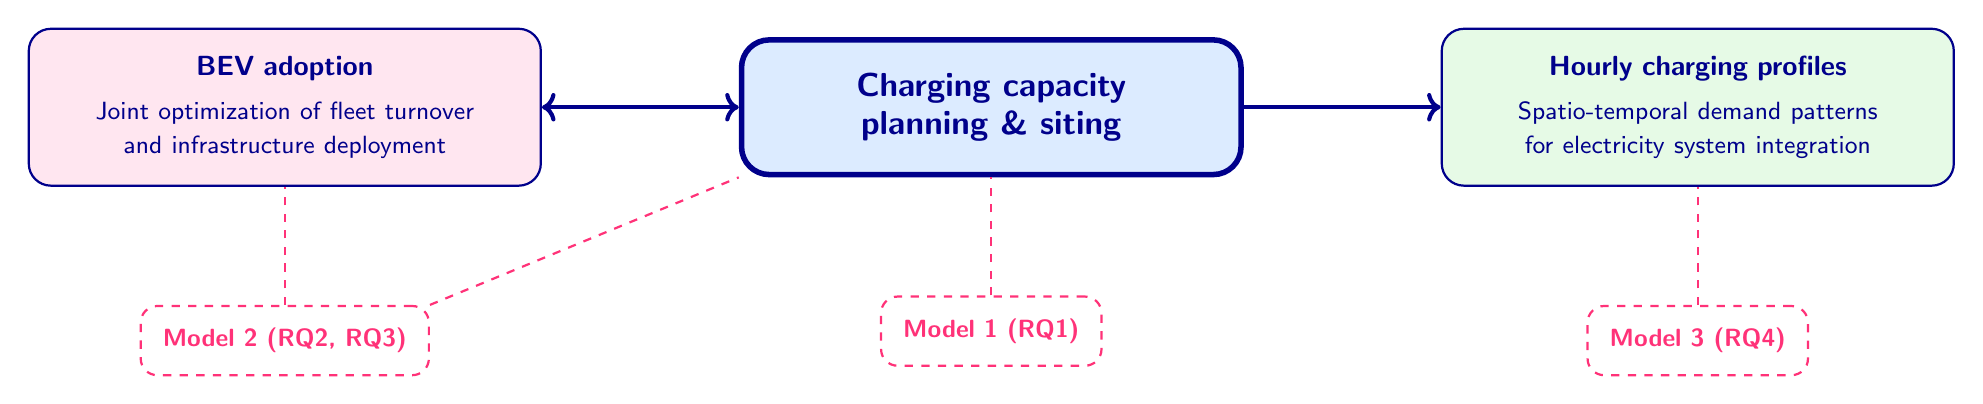
\begin{tikzpicture}[
    node distance=1.2cm,
    corebox/.style={
        draw=darkblue, line width=2pt, rounded corners=10pt,
        text width=5.5cm, align=center, inner sep=12pt,
        font=\large\bfseries, text=darkblue,
        fill=lightblue
    },
    sidebox/.style={
        draw=darkblue, thick, rounded corners=8pt,
        text width=5.8cm, align=center, inner sep=10pt,
        font=\normalsize, text=darkblue
    },
    modelbox/.style={
        draw=pinkdash, dashed, thick, rounded corners=6pt,
        inner sep=8pt, font=\small\bfseries, text=pinkdash
    },
    arrow/.style={-{Stealth[length=3.5mm]}, darkblue, line width=1.5pt},
    rqlabel/.style={font=\small\bfseries, text=darkblue}
]

% CORE - center
\node[corebox] (core) {Charging capacity\\planning \& siting};

% LEFT - BEV adoption
\node[sidebox, left=2.5cm of core, fill=lightpink] (adoption) {
    \textbf{BEV adoption}\\[4pt]
    \small Joint optimization of fleet turnover and infrastructure deployment
};

% RIGHT - Charging profiles
\node[sidebox, right=2.5cm of core, fill=lightgreen] (profiles) {
    \textbf{Hourly charging profiles}\\[4pt]
    \small Spatio-temporal demand patterns for electricity system integration
};

% Arrows
\draw[arrow, <->] (adoption.east) -- (core.west);
\draw[arrow, ->] (core.east) -- (profiles.west);

% Model labels below
\node[modelbox, below=1.5cm of adoption] (m2) {Model 2 (RQ2, RQ3)};
\node[modelbox, below=1.5cm of core] (m1) {Model 1 (RQ1)};
\node[modelbox, below=1.5cm of profiles] (m3) {Model 3 (RQ4)};

% Dashed lines connecting models to their boxes
\draw[pinkdash, dashed, thick] (m2.north) -- (adoption.south);
\draw[pinkdash, dashed, thick] (m1.north) -- (core.south);
\draw[pinkdash, dashed, thick] (m3.north) -- (profiles.south);

% Additional: Model 2 also connects to core
\draw[pinkdash, dashed, thick] (m2.north east) -- (core.south west);

\end{tikzpicture}
\end{document}
